\section{Multithreading}
Since the synchronization method described in Sec. \ref{sec:sync_algo}
relies heavily on the arrival timestamps $\atime{}$ it is important
that incoming images are time stamped immediately before further
processing. This section describes how multithreading can be used to
accomplish this.

Fig. \ref{fig:multithreading} provides an overview of the
architecture. A separate polling thread is started for each camera,
and performs a blocking call to the FLIR/PointGrey FlyCapture driver API
to receive an image for the respective camera.
When the call returns, the polling thread immediately records the
arrival time stamp, updates the exposure settings if required, and
adds the image, together with the arrival time stamp, to the front of
a global synchronization queue. This is a very light weight operation
and requires only a short amount of time, thus ensuring that there is
very little resource contention, and none of the polling threads are
prevented from immediately entering the next blocking driver call.

A single synchronization thread operates on the synchronization
queue and computes the frame time stamps as described in
Sec. \ref{sec:sync_algo}. Finally, the time stamped frames are entered into a 
per-camera queue that compresses and publishes the image, thereby
making it available to subscribers on the ROS network.

\label{sec:multithreading}
\begin{figure}[ht]
	\centering
	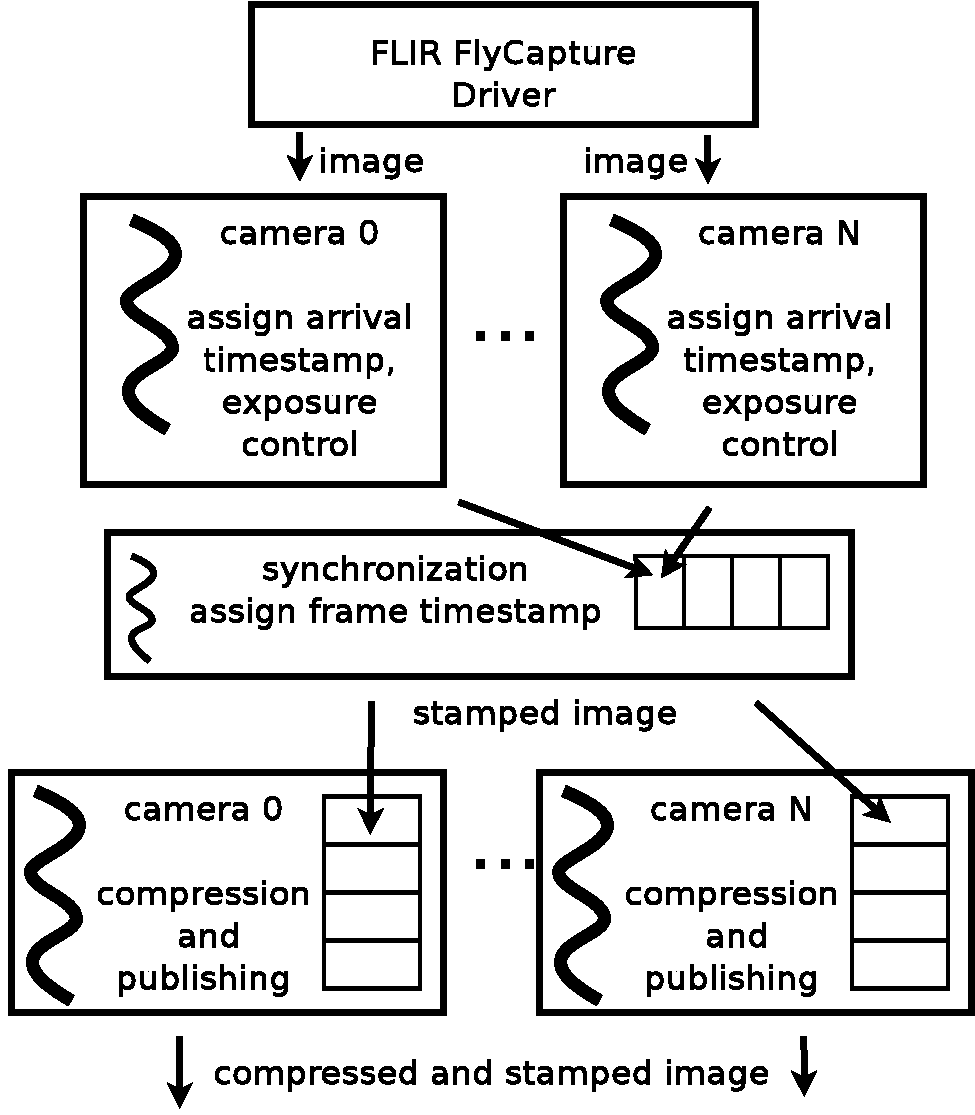
\includegraphics[width=\linewidth]{figures/threading.pdf}
        \caption{Multithreading: one thread per camera receives the
          image from the driver with a blocking call, puts on the
          arrival timestamp, updates exposure settings, and enqueues
          the image for the synchronization thread to process. Once
          the frame time stamp has been determined, the image is
          entered into a per-camera queue for compression and publishing.}
    \label{fig:multithreading}
\end{figure}
